\chapter{Convolutional neural networks}
\label{cnn}

% \setcounter{secnumdepth}{1}

Although it is assumed that the reader has sufficient prior knowledge of artificial neural networks and convolutional neural networks, this part briefly introduces convolutional neural networks, their layer types and few selected architectures. 

For better understanding of the topic, it is recommended to take a look at the holy book of deep learning, \cite{dl}.

\section{Introducing convolutional neural networks}
\label{understanding-cnn}

If you try to find an introduction to \zk{CNN}s on the internet, you may bump into a common statement that \zk{CNN}s are neuroscience-based deep neural networks using convolution and presumpting the input is an image. It is not exact. 

Though images are the most common input, according to \cite{dl}, \zk{CNN}s presumpt the input has a grid-like topology; apart from the computer vision, other applications include  for example natural language processing (as in \cite{cnn-nlp}) or anything representable as a grid-like topology (audio waveform as 1-D grid, RGB images as multichannel 2-D, CT scan as 3-D, etc.). 

A paradox inexactness is the term \textit{convolution} as in mathematical meaning, many \zk{CNN}s implement cross-correlation instead of real convolution. Cross-correlation may be seen as convolution without a kernel flipping. The reader can get more mathematical insight about the difference and harmlessness of this change from \cite{dl}. 

It is true that \zk{CNN}s are based on a neuroscience. They are inspired by Nobel prize laureates Hubel's and Wiesel's research on mammalian vision systems (firstly cats in \cite{hubel-cats1} and \cite{hubel-cats2}, later monkeys in \cite{hubel-monkeys}). Hubel and Wiesel found that some neurons (sorted in columns) strongly respond to specific to specific edge-like patterns but just a bit to other patterns. 

The eye stimulus on the retina is transferred through the optic nerve and the lateral geniculate nucleus into the primary visual cortex (sometimes referred to as V1), a part of the visual cortex located in the posterior pole of the occipital lobe. The primary visual cortex is organized in a 2-D spatial map representing visual stimuli from the retina and contains two cell types, simple cells and complex cells. Simple cells purpose is to compute a linear function (although some counterarguments against the linearity have been raised, see \cite{simple-cells}) of the image in a spatially localized field, while complex cells operations are to some extent position and lighting invariant. 

\section{Layer types}
\label{layers}

While the common approach in image processing of classical \zk{ANN}s is to vectorize the input, \zk{CNN}s emulate the neuroscientific approach outlined in chapter \ref{understanding-cnn} using feature maps (each color channel is a feature map). \zk{CNN}s profit from the fact that pixels in an image are ordered according to some structure. That allows neurons in layers to be connected just to certain region instead of heavily arduous fully-connected architecture. 

\zk{CNN}s consist from many layers with different functions. In the following, individual layer types are briefly described. 

\subsection{Convolutional layers}
\label{conv-layers}

The first layers through which is the input passed are convolutional layers. So, firstly, what is the convolution? 

In the geomatics field, we very often encounter the term \textit{kernel}. Kernel can be seen as a matrix (or a window) sliding across all the image pixels. The pixels contained in this window are a receptive field. As both the kernel and the receptive field are matrices of the same shape, in each position element wise multiplication is computed and outputed as an output matrix element. Because after such a filtering, the output matrix contains a 2-D activation map (a map where each position values say with witch probability the requested feature is on that position in the original image), the output is called a \textit{feature map}. Kernels / filters are the subject of training. 

In case of stride 1 and without zero-padding, the feature map is naturally of shape $[original\_width - kernel\_width + 1] \times [original\_height - kernel\_height + 1]$. An example may be seen in figure \ref{fig:conv}. 

\begin{figure}[H]
   \centering
	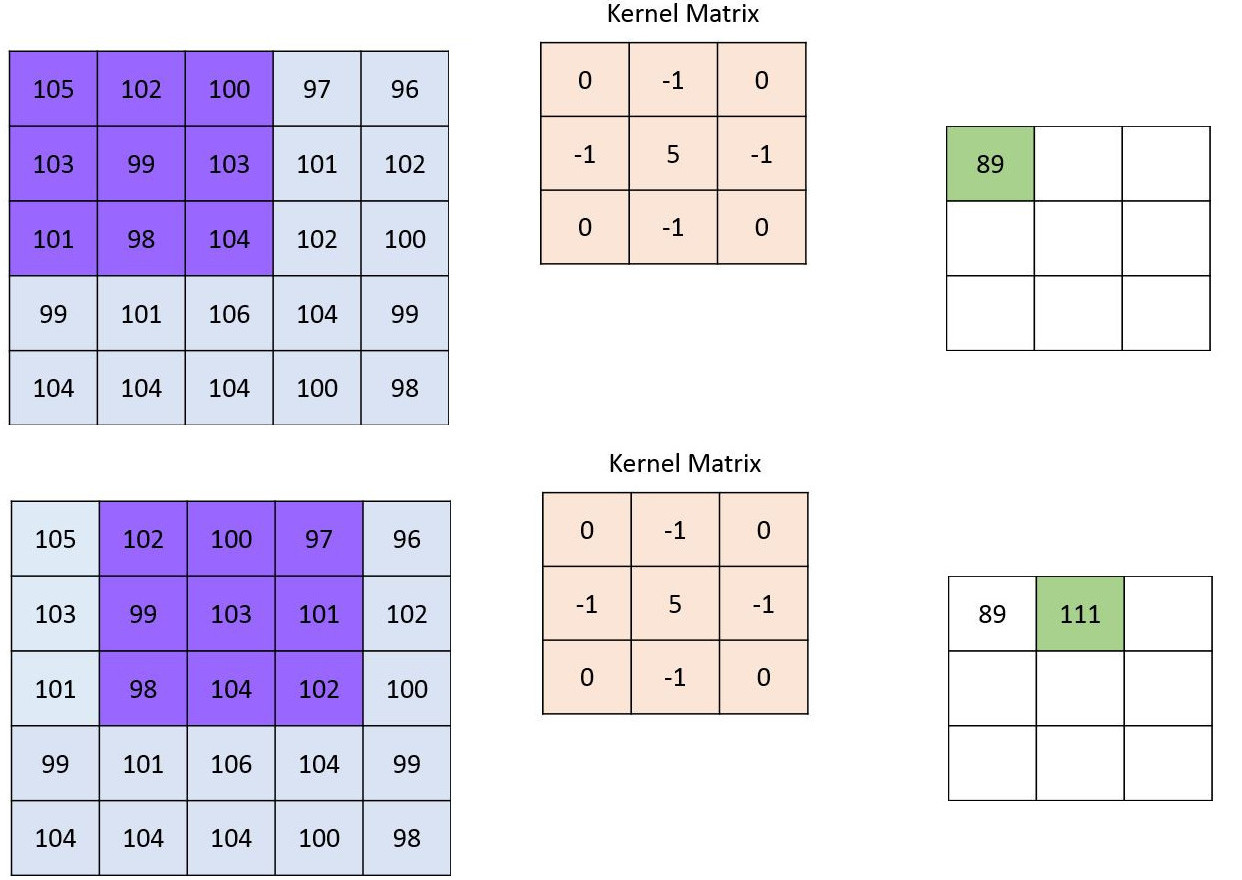
\includegraphics[width=.4\linewidth]{./pictures/conv.jpg}
	\caption[Kernel convolution]{Two steps of kernel convolution}
      \label{fig:conv}
\end{figure}

With convolution, we reduce both computational requirements and a threat of overfitting by using local connections (representing weights) between input and output. However, these connections are local only in two dimensions, in width and height of the input; these connections have to be full along the channels depth - e.g. in RGB images, the last dimension of connections is always 3. Different is it with the output; its third dimension (\textit{depth}) is determined by the number of neurons referencing the same spatial location, e.g. by the number of kernels we use. 

In chapter \ref{understanding-cnn}, translational invariance was mentioned. In convolutional layers, the first step to this invariance was achieved by another huge parameter reduction, by parameter sharing. Idea of parameter sharing raised from the premise that when one feature is useful in one location, it could be useful also in another one. This simple presumption which works except for for example centered special structures allows sharing a set of parameters throughout the whole depth slice. 

Using the parameters from \cite{cnn-classification} as an example, assumpt that the feature map has size $55 \times 55 \times 96$ and we apply it on images of size $227 \times 227 \times 3$\footnote{The paper claims that the images were of size $224 \times 224 \times 3$, but it is assumpted that it was either a typo or authors forgot to mention a zero-padding} using kernels of size $11 \times 11 \times 3$. Sharing parameters within a depth slice, we can reduce the parameter amount from $55 * 55 * 96 * (11 * 11 * 3 + 1)$ to $96 * (11 * 11 * 3 + 96)$ (1 and 96 are biases), it means from more than 105 millions to less than 35 thousands. Speaking only about the first layer. I believe that this example said it all. 

An inquiring reader may raise a question: In the chapter name, there is a plural. What happens in deeper layers? 

Their input is the previous layer output. Output of the first layer is the feature map of the lowest level features. As was already mentioned, each neuron of the next layer is connected with some local neighbourhood and with everything along the third dimension; and because the third dimension of the output is formed by stack of filters / kernels of the first layer, each second layer neuron is connected to all detected features in some location and its neighbourhood. The result? Output feature map from the second layer contains higher level features (simple combinations of the low level ones, like triangles or squares, simply combinations of some edges, curves, etc.). The next layer will output again higher level features and in the end, we may have very specific features like cars, reflective heliports or art deco swimming pools. This principle is illustrated in figure \ref{fig:deconvnet} using a deconvolutional network, a technique described in chapter \ref{zfnet}.

\subsection{ReLU layers}
\label{relu-layers}

Since the real data we are using to train our \zk{CNN}s are mostly non-linear, it is useful to introduce some non-linearity into the network. In the past, functions like hyperbolic tangent or sigmoid were used, but Rectified Linear Unit (\zk{ReLU}) has been found to be trained faster and mitigate the vanishing gradient problem (problem of slow training of low layers due to the exponential decrease of the gradient). 

\zk{ReLU} output is defined by a function:

$f(x) = max(0, x)$

After applying the \zk{ReLU} function to of the input values, we have a feature map where all negative values of the input were changed to zero. This output is called \textit{rectified feature map}. 

\subsection{Pooling layers}
\label{pooling}

Eventhough the input size reduction might already be included in convolutional layers, it is very common to include another layers with this purpose. Because of this purpose, they are called \textit{pooling layers} or \textit{subsampling layers} (they can do both downsampling or upsampling). 

Pooling layers work again with a kernel. But this time, the stride is bigger than one which is quite uncommon for convolutional layers. It means that when we use a pooling layer with kernel of size 2$\times$2 and stride 2, the output will be half in first two dimensions (the third one is preserved). One pooling like this reduces parameters by 75 percent. 

Aside from the parameter reduction, there are two more positive effects. Because of the detail mute, it reduces a threat of overfitting and it also strengthens the shift invariance. The advantage of pooling layers is also the fact that they do not introduce no new parameters to the network. 

The function for the kernel can vary, but the most-used one is max-pooling\footnote{Choosing the biggest value from those overlaid by the kernel.} having the advantage that it does not matter where in the region was the value detected. Other customary approaches apply average (compared with max-pooling in \cite{avg-pooling}), $L2$ \cite{l2-pooling} or Stochastic pooling \cite{stoch-pooling}. Also used kernel size and stride vary, the most common ones are 2$\times$2 with stride 2 and 3$\times$3 with stride 2. 

Also, architectures without pooling layers are not so uncommon today. One research on this approach can be seen in \cite{all-conv-net}. It introduces an architecture called \textit{all convolutional net} where the subsampling may be done by increasing the stride and compares it with other approaches. 

\subsection{Normalization layers}
\label{norm-layers}

Besides neural exhibition, neural inhibition is also found in the human brain. These doors of perception stay half-closed and filter or inhibit human receptions.

Normalization layers can be seen as an attempt to imitate this structure, but there are more reasons for these layers in deep learning. As was written above, input for higher (deeper) layer is the output of lower level. It means that the highest (deepest) layer input is dependent on the first layer output. Because functions of layers are changed each training step, a small change of the first layer output may have huge effect on the last layer input and therefore also on the last layer output, which may lead to completely wrong behaviour of deeper layers. This problem is called a \textit{covariate shift} or, following terminology from \cite{batch-norm}, an \textit{internal covariate shift}. 

This change in the distribution can be to some extent reduced by using a small learning rate and right initialization of the network. Because small learning rate radically extends the training time, other solutions were needed. Normalization layers. 

One of the most widely used approaches is called \textit{batch normalization} \cite{batch-norm}. In \zk{CNN}s, it is common to use batches (or mini-batches) of training examples instead of one-at-a-time as the computation parallelism saves time. Batch normalization computes a mean and variance over a batch using the distribution of the summed neuron input and whiten\footnote{Set means equal to zero and variances unit; idea proposed in \cite{tricks}.} it for each training batch. According to \cite{batch-norm}, it reduced the number of training steps 14 times allowing the user to use much higher learning rate and being less careful about initialization.

Another types of normalization layers include local response normalization or $L2$ normalization.

\subsection{Fully connected layers}
\label{fc-layers}

As their name prompts, fully connected (\zk{FC}) layers are layers where each neuron in a layer is connected to each neuron of the previous layer. Their activations can be seen simply as a matrix multiplication enhanced by a bias.  

The purpose of \zk{FC} layers is to take the high-level feature map as an input and return a classification vector as an output. Each value in the output refers to one class occurrence, e.g. the length of the output vector is $n$ where $n$ is the number of classes. \zk{FC} layers are not so hard to train to use non-linear combinations of features in input which is widely used whereas the combinations of high-level features are the things we are looking for. For example, if we are looking for a platypus, the last layer output will have high values in the neurons that represent things like a duck-like snout, four legs, flat tail or a calcaneous spur; if we are looking for a jelly, we will most probably not be interested in any of these features. 

Using popular \textit{softmax} classifier\footnote{Softmax transforms a vector of real-valued values to a vector of values between zero and one that sum to one.}, the output is a vector of probabilities representing each class. Other classifiers like \zk{SVM} can also be used. 

Fully connected layers are sometimes referred to also as \textit{dense layers}.

\section{Architectures of convolutional neural networks}
\label{cnn-architectures}

It is generally resolved\footnote{Roots of \zk{CNN}s are in the end of eighties, but the breakthrough came in nineties.} that the history of succesful \zk{CNN}s started in 1998 when Yann LeCun and his team published the paper Gradient-Based Learning Applied to Document Recognition \cite{lenet5}. Although it is just twenty years, \zk{CNN}s have made tremendous progress. During this period, a plenty of various architectures was proposed, more or less succesful.

Because some background of the \zk{CNN} architectures evolution could help in understanding \zk{CNN} fundamentals and deepens the insight into research and decisions made for this thesis, few of the most influental architectures will be mentioned in the following chapters.

In this chapter, ImageNet Large Scale Visual Recognition Challenge (\zk{ILSVRC}) will be mentioned several times as it is something like a fuel for computer vision progress with which are \zk{CNN}s inseperably connected. For the topic of this thesis, it should be enough to say that \zk{ILSVRC} is a competition in visual recognition including many diverse tasks, for more informations and results take a look into \cite{ILSVRC} which was used also during writing this chapter.

\subsection{LeNet-5} %
\label{lenet}

Nobody would argue that the fundamental architecture is the one from the paper Gradient-Based Learning Applied to Document Recognition mentioned above, the one called LeNet-5. It was proposed in \cite{lenet5} and due to the lack of GPU and insufficience of CPUs, its convolutional, computationally economical approach ensured the architecture a huge success and usage for example in character recognition (reading zip codes, checks). 

In figure \ref{fig:lenet}, we can see the architecture of LeNet-5. It contains many features mentioned in chapter \ref{layers}. It consists of convolutional, pooling (subsampling) and \zk{FC} layers and it also introduced the non-linearity into the network using hyperbolic tangent or sigmoids. Its two convolutional layers (C1 and C3) apply $5 \times 5$ convolutional filters with stride $1$ and its two pooling layers (S2 and S4) apply $2 \times 2$ average-based filters with stride $2$. The architecture is finished with two \zk{FC} layers; one is needed to learn the non-linear combinations of high-level features, the other one to classify the results\footnote{Gaussian connections are used here instead of softmax mentioned in \ref{fc-layers}. They are based on Euclidean Radial Basis Function and described in \cite{lenet5}.}.

\begin{figure}[H]
   \centering
	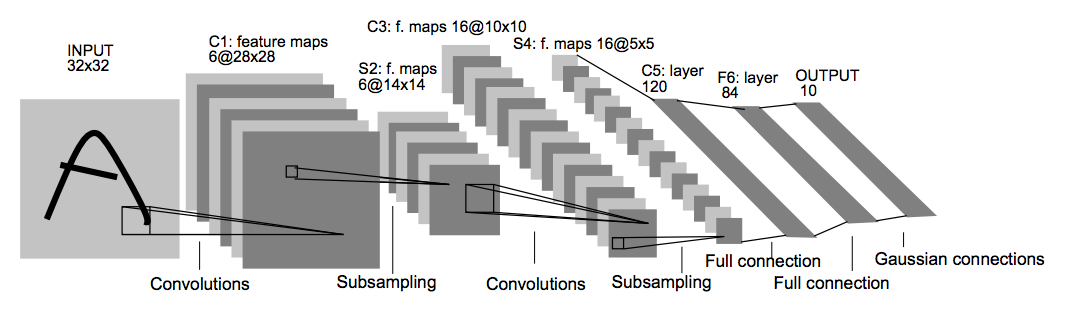
\includegraphics[width=\linewidth]{./pictures/lenet.png}
	\caption[LeNet-5 architecture]{LeNet-5 architecture schema, source: \cite{lenet5}}
      \label{fig:lenet}
\end{figure}

LeNet-5 made the first important step for \zk{CNN}s and a big step for \zk{ANN}-based computer vision generally. It explained that taking an input as individual values - besides its speed and computation problems - does not use the advantage of spatial correlations within the input. 

%\subsection{Dan Ciresan Net}
%\label{ciresan}

% first with GPU
% 2010
% if uncommented, change begining of AlexNet

\subsection{AlexNet} %
\label{alexnet}

As was mentioned, LeNet-5 became very succesful first step. Nevertheless, until 2010s, development of \zk{CNN}s was out of the main spotlight. Although there were few important events like Dan Ciresan using GPU neural nets in 2010, the main one happened in 2012, when Alex Krizhevsky came with something like a deeper version of LeNet in \cite{cnn-classification} and called it AlexNet. That year, AlexNet won the \zk{ILSVRC}\footnote{AlexNet won it by a great margin with top 5 error of 16.4 \% compared to the second place with 26 \%.}.

Krizhevsky benefited from years of progress bringing more computing power and more data to be trained on. This well timed entree allowed him to use a deep architecture containing about sixty millions parameters, \zk{ReLU} layers, overlapping max pooling and dropout\footnote{A technique used to prevent overfitting proposed in \cite{dropout}. Dropout selectively ignore individual neurons during training.}. AlexNet also included a stack of convolutional layers instead of previous approach, where each convolutional layer was followed by a pooling layer. 

The computation was done on GPU (NVIDIA GTX 580) which allowed him to use larger datasets consisting of more and larger images as well as fastened the training. The separate GPU approach is indicated in figure \ref{fig:alexnet} by upper and lower part of the image as two different GPU processes; it can be seen that the interaction between two GPUs happens only at certain layers. 

\begin{figure}[H]
   \centering
	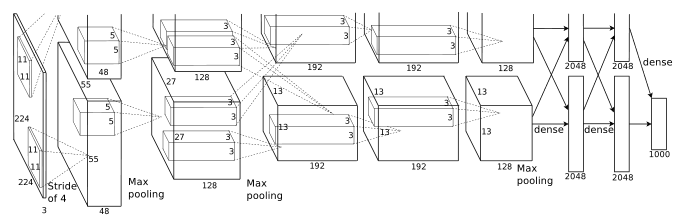
\includegraphics[width=\linewidth]{./pictures/alexnet.png}
	\caption[AlexNet architecture]{AlexNet architecture schema, source: \cite{cnn-classification}}
      \label{fig:alexnet}
\end{figure}

If LeNet-5 represents the first step of \zk{CNN}s, AlexNet is the first marathon. After its success, \zk{CNN}s became the bleeding edge in both deep learning and computer vision. 

% CS231n about zero-padding

\subsection{ZF Net}
\label{zfnet}

After the success of AlexNet, the number of \zk{CNN}s competing in the ImageNet Large Scale Visual Recognition Challenge (\zk{ILSVRC}) noticeably increased. Matthew Zeiler and Rob Fergus built an architecture called ZF Net and won the \zk{ILSVRC} 2013 with top 5 error rating of 11.2 \%. 

ZF Net architecture was based on AlexNet and described in \cite{zf-net}. Because it was believed that the $11 \times 11$ filtering in the first layer of AlexNet skipped too much information, it was replaced with a filter of size $7 \times 7$ with a decreased stride. Besides the parameter tweaking, the size of the middle convolutional layers expanded and the cross-entropy loss function was used as well as stochastic gradient descent with a mini-batch size of 128. The architecture can be seen in figure \ref{fig:zf-net}.

\begin{figure}[H]
   \centering
	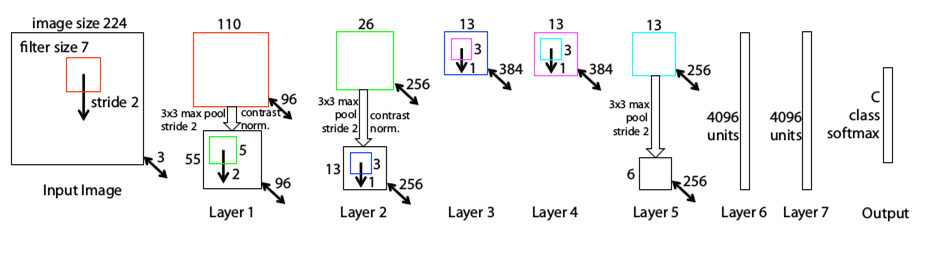
\includegraphics[width=\linewidth]{./pictures/zf-net.png}
	\caption[ZF Net architecture]{ZF Net architecture schema, source: \cite{zf-net}}
      \label{fig:zf-net}
\end{figure}

An important feature was introducing a technique mapping features from feature maps back to pixels, due to its character this technique is called a \textit{deconvolutional network}. During the forward pass, activations are computed at each level of \zk{CNN}s; when we want to observe a certain feature of a certain layer, we pass it back through the preceding layers. In this back pass, operations are in another direction (pooling is changed to unpooling, downsampling to upsampling etc.) until the input layer is reached. It gives the user an idea of what kinds of structures are recognized in the certain feature map. A visualization of 5 layers illustrating the way from low-level features like edges or colours to high-level features like dog faces or flowers can be seen in figure \ref{fig:deconvnet}.

\begin{figure}[H]
   \centering
	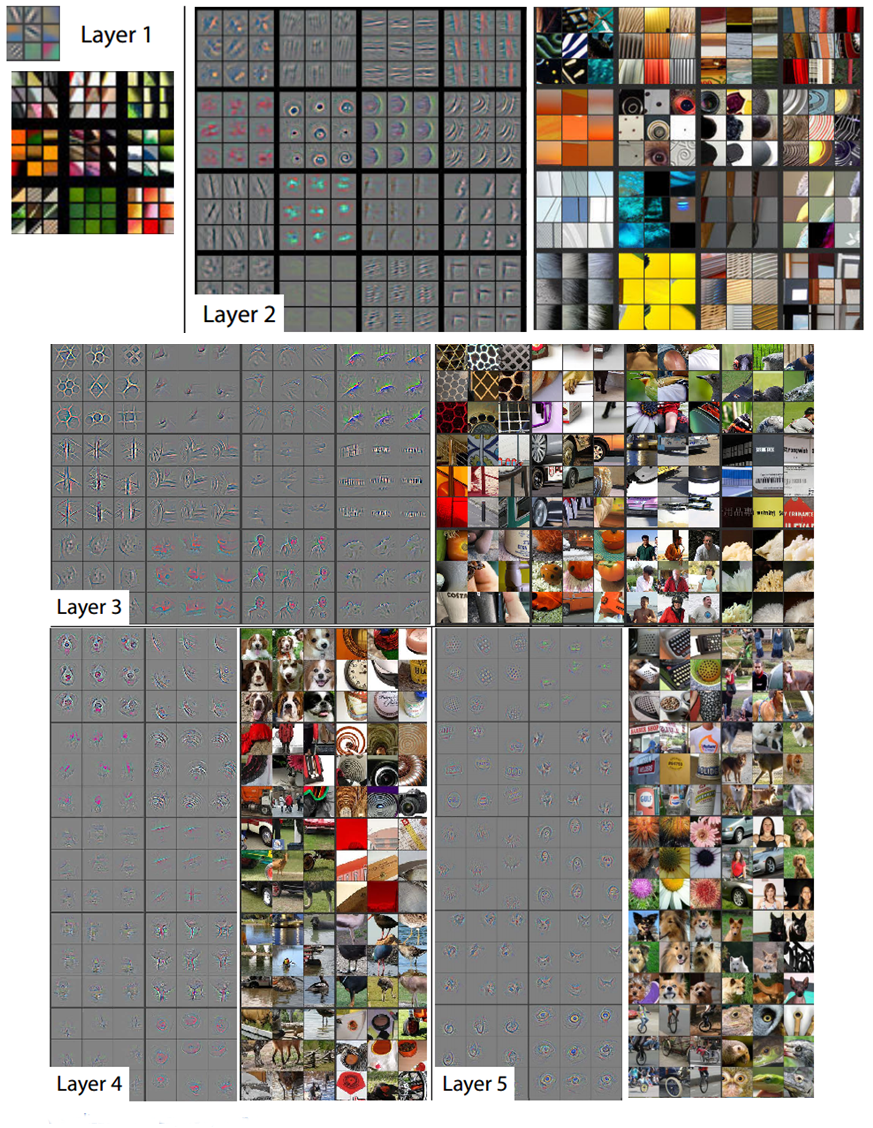
\includegraphics[width=\linewidth]{./pictures/deconvnet.png}
	\caption[Deconvolutional network]{Visualization of 5 feature maps through deconvolutional networks, source: \cite{zf-net}}
      \label{fig:deconvnet}
\end{figure}

Thanks to its modifications, it was enough to train ZF Net on only 1.3 million images instead of 15 million images used with AlexNet. However, the training took 12 days instead of 5 or 6 and was stopped after 70 epochs. The training ran on a single GPU.

However, in \cite{zf-net}, Zeiler and Fergus did more than just bring new architecture. They summarized why the time of \zk{CNN}s had just come and tried to deepen the general knowledge behind these models, where especially the deconvolution visualization of feature maps can be called a missionary work.

\subsection{VGG Net}
\label{vgg}

\zk{ILSVRC} 2014 brought new interesting architectures. Although VGG Net, an architecture proposed by Visual geometry group of the University of Oxford in \cite{vgg}, was not the winning architecture, it reached the error rate 7.3 \% even with its \textit{simplicity-in-the-first-place} architecture.

Authors experimented with different architectures with number of layers between 11 and 19 (see figure \ref{fig:vgg} for their parameters) and chose 16-layer architecture homogenously using only $3 \times 3$ filters with stride and zero padding of size 1 to preserve the spatial resolution after convolution interleaved with maxpooling layers with stride 2. They found that when we use multiple convolutional layers with smaller kernels in a row, it emulates the effect of larger kernels while still retaining advantages of smaller kernels; it means that 3 layers with kernel $3 \times 3$ emulate the effect of 1 layer with kernel $7 \times 7$, decrease the number of parameters and allows the user to implement three ReLU layers instead of one, exactly the advantage VGG Net used. It has to be said that the number of parameters was still enormous reaching almost 140 millions and in the following architectures, this problem caused by \zk{FC} layers had to be solved to reduce the time consumption.

VGG Net also enlarges the number of filters after each maxpool layer as can be seen in figure \ref{fig:vgg}; the idea of decreasing spatial dimensions but increasing the third (depth) dimension was shown to be very important as well as the depth (number of layers) of the network. During the mini-batch gradient descent based training, a scale jittering was used for the data augmentation to train the model to recognize objects at different scales. The training took two to three weeks depending on the architecture and was carried out by 4 NVIDIA Titan Black GPUs.

\begin{figure}[H]
   \centering
	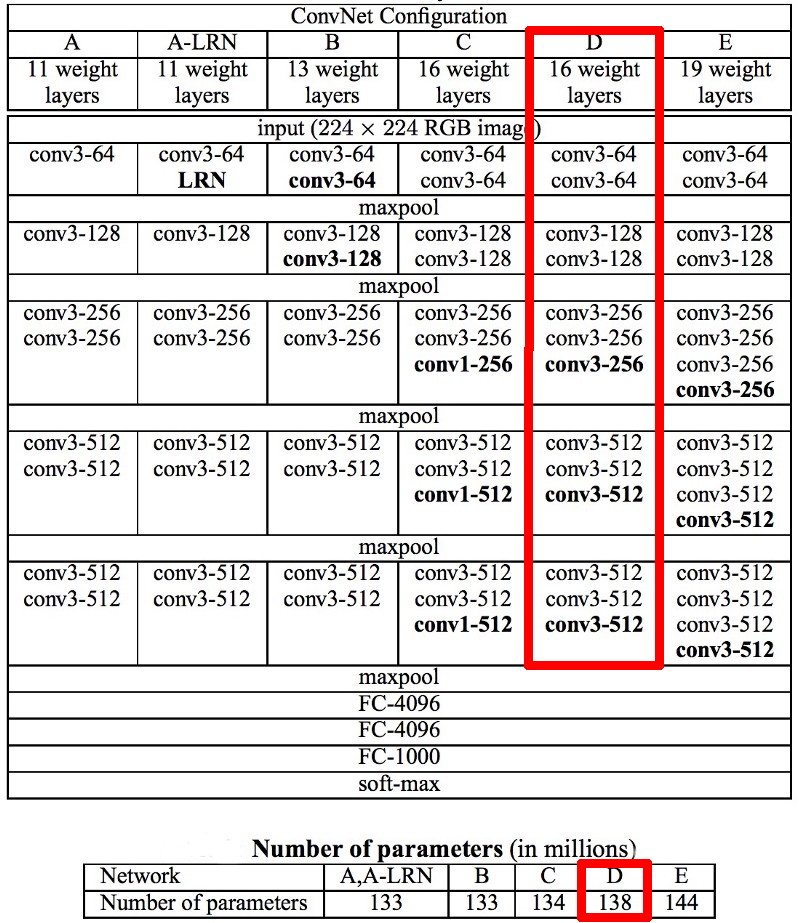
\includegraphics[width=0.8\linewidth]{./pictures/vgg-net.png}
	\caption[VGG Net networks]{Different architectures of VGG Nets and the chosen one, source: \cite{vgg}}
      \label{fig:vgg}
\end{figure}

% localization regression pp 10 of {vgg}
% Caffe

% \subsection{Network-in-network}
% \label{nin}

% 1x1 convolutions
% if uncommented, change footnote in googlenet

\subsection{GoogLeNet}
\label{googlenet}

And now for something completely different. Authors of GoogLeNet, the winning architecture of \zk{ILSVRC} 2014 with a top 5 error rate of 6.7 \%, proposed in \cite{googlenet} another approach, instead of at the architecture simplicity aiming at the computational simplicity.

\begin{figure}[H]
   \centering
	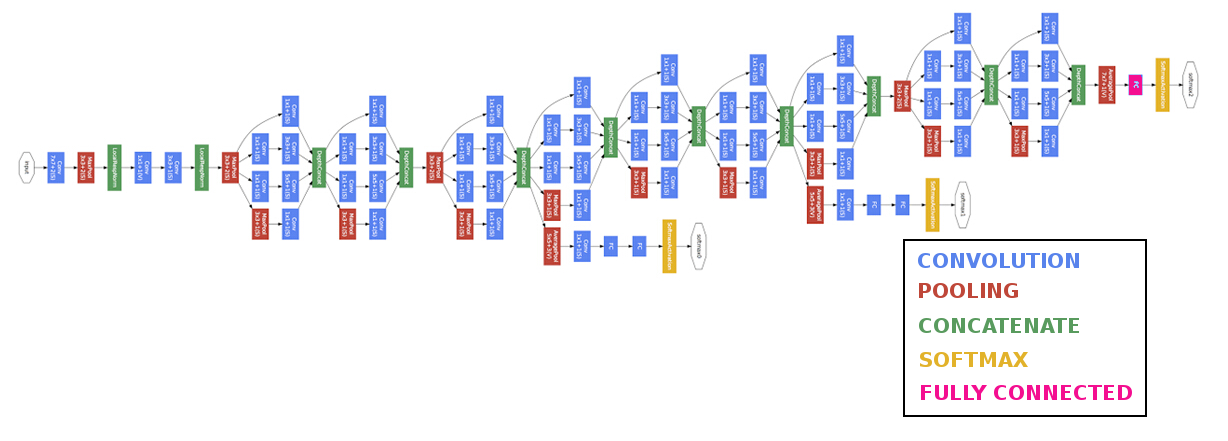
\includegraphics[width=\linewidth]{./pictures/googlenet.png}
	\caption[GoogLeNet networks]{GoogLeNet network schema, source: \cite{googlenet}}
      \label{fig:googlenet}
\end{figure}

In figure \ref{fig:googlenet}, we can see parallel blocks. Authors found that the sequential queue of layers increases a computational and memory cost a lot, so they proposed a module called \textit{Inception}. The naïve idea behind the Inception module is illustrated in figure \ref{fig:inception-naive} and is quite simple: Why should we stack the layers in a sequence, when we can perform them in a parallel? Though the idea behind was not bad, this naïve version ended in an enormous depth (size of the third dimension) of the output after the concatenation into a single vector.

\begin{figure}[H]
   \centering
	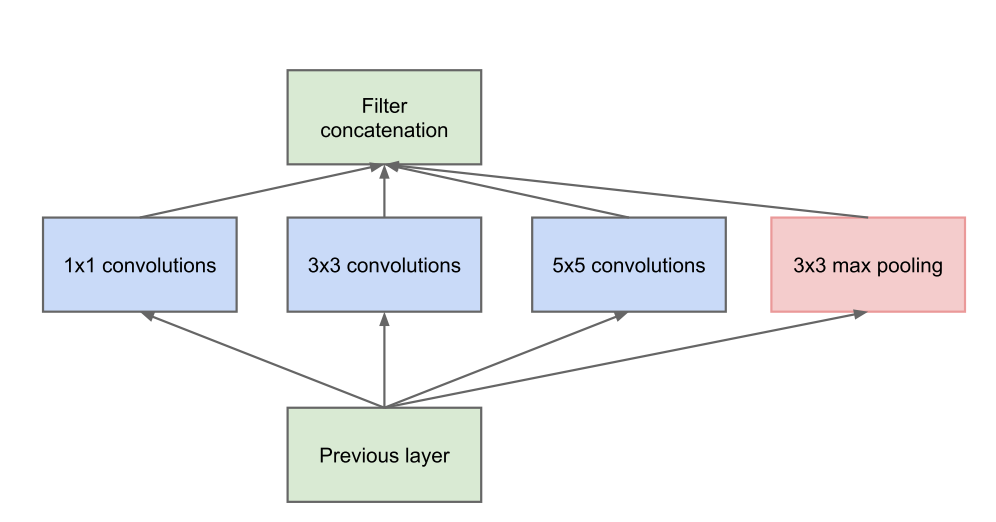
\includegraphics[width=0.8\linewidth]{./pictures/inception-naive.png}
	\caption[Inception module, naïve idea]{Naïve idea of Inception module, source: \cite{googlenet}}
      \label{fig:inception-naive}
\end{figure}

As can be seen in figure \ref{fig:inception-full}, authors solved the depth problem by adding $1 \times 1$ convolutional layers, sometimes referred to as \textit{network in network}\footnote{The alias of this approach was derived from the architecture called Network-in-network proposed in \cite{nin} and presenting the advantages of $1 \times 1$ convolutions.}. Usage of 10 $1 \times 1$ filters outputs a volume with two dimensions equal to the input dimensions and the third one equal to 10. The depth of input for bigger kernels is thus \textit{pooled} to the defined size, while allowing also to use one more ReLU layer after the $1 \times 1$ convolution. This process is sometimes called a \textit{bottleneck} (likewise the $1 \times 1$ layer is sometimes called a \textit{bottleneck layer}).

\begin{figure}[H]
   \centering
	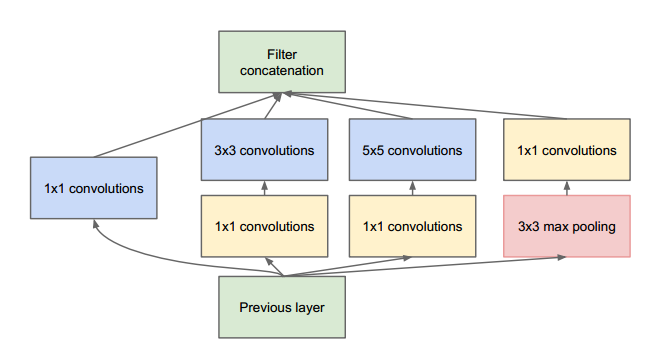
\includegraphics[width=0.8\linewidth]{./pictures/inception-full.png}
	\caption[Inception module, full]{Inception module with dimensionality reduction, source: \cite{googlenet}}
      \label{fig:inception-full}
\end{figure}

The parallelized architecture used over 100 layers while the real depth of the full network was just a fraction of this number and it used only 7 Inception modules. Authors also get rid of unnecessary \zk{FC} layers and instead used an average pooling which concluded in twelve times fewer parameters than AlexNet. Their architecture also decreased the threat of overfitting. In \cite{googlenet}, authors claimed that the network was trained \textit{using few high-end GPUs within a week}.

Time from time, updated versions are published. Interested readers may try to find architectures like Inception V2, Inception V3 and higher.

\begin{figure}[H]
   \centering
	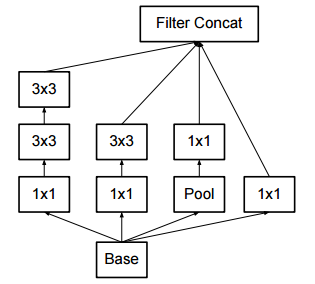
\includegraphics[width=0.3\linewidth]{./pictures/inception-v2.png}
	\caption[Inception V2]{Inception V2 used the idea described already in chapter \ref{vgg} about replacing $5 \times 5$ convolution with two $3 \times 3$ convolutions, source: \cite{inception-v2}}
      \label{fig:inception-v2}
\end{figure}

%\subsection{Inception V3}
%\label{inception}

\subsection{ResNet}
\label{resnet}

In the above described architectures, a trend of going deeper can be noticed. Microsoft Research team noticed it too and in \cite{resnet}, they proposed much deeper architecture than previous ones. This architecture was called ResNet, contained 152 layers and won \zk{ILSVRC} 2015 with an error rate of 3.6 \% beating even humans with their error rate of circa 5 -- 10 \%.

Although the depth was quite revolutionary, it was not the most innovative thing of ResNet. Neither was the usage of batch normalization as described in \cite{batch-norm} after each convolutional layer. The most innovative thing of ResNet was a structure called a \textit{residual block}. In 2011, Pierre Sermanet and Yann LeCun proposed in \cite{bypass} a notion to \textit{bypass} a layer. ResNet used this design with a richer mind and as can be seen in figure \ref{fig:res-block}, they bypassed two layers.

\begin{figure}[H]
   \centering
	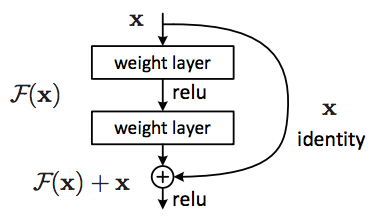
\includegraphics[width=0.4\linewidth]{./pictures/residual-block.png}
	\caption[Residual block]{A residual block schema, source: \cite{resnet}}
      \label{fig:res-block}
\end{figure}

Bypassing two layers (a term \textit{skip connections} is not uncommon) gives much better improvements than the single layer bypass. But what exactly happens during the bypass? In traditional \zk{CNN}s, only the $F(x)$ is computed. It means that the next layer does not have the real connection to the original input, but only to this transformed output, $F(x)$. When we bypass the block input $x$ after 2 layers, we can add it to $F(x)$ which represents a change this time. By the addition, we get a mildly altered representation of the input. Authors of ResNet declared that it is easier to optimize this referenced mapping instead of the unreferenced one. Another advantage is that with addition operations, the backward propagated gradients will flow easier through the structure. Because the mapping was referenced using residuums, it is sometimes referred to as a \textit{residual mapping}.

Authors experimented with diverse depths of the architecture counting 18, 34, 50, 101 and 152 layers. During these experiments, authors found a problem in number of parameters in deeper architectures. However, they found a solution by following the design of bottleneck layers described in chapter \ref{googlenet}: They redesigned the residual block into a bottleneck block. This block reduced the number of features usually to one quarter by using $1 \times 1$ convolutions and was implemented into ResNet-50 and higher.

\begin{figure}[H]
   \centering
	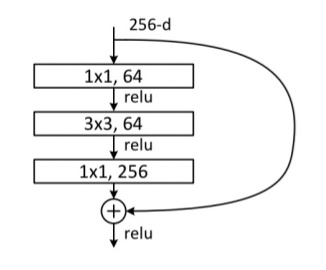
\includegraphics[width=0.4\linewidth]{./pictures/bottleneck-block.jpg}
	\caption[Bottleneck block]{A bottleneck block schema, source: \cite{resnet}}
      \label{fig:bottleneck-block}
\end{figure}

Mentioned experiments contained one more interesting event. A creation of a real monster, a 1202-layer network. Surprisingly, this network got a lower accuracy during tests. Authors argued that this is because of overfitting.

8 GPUs were used for the training of ResNet-152 and the process took something between two and three weeks.

The continuation of ResNet can be found for instance in an architecture called ResNeXt. Saining Xie and his team proposed ResNeXt in \cite{resnext} and it combines ResNet with modularized parallel pathways similar to those described in chapter \ref{googlenet}.

% \subsection{SqueezeNet}
% \label{squeezenet}

% \subsection{ENet}
% \label{enet}